\documentclass[12pt]{article}
\usepackage[utf8]{inputenc}
\usepackage{graphicx}
\usepackage{listings}
\usepackage{wrapfig}
\usepackage{subfigure}
\usepackage{hyperref}
\usepackage{amsmath}
\usepackage[margin=1in]{geometry}
\usepackage[htt]{hyphenat}

\title{Project Documentation:\\Browser-Based 3D Turtle}
\author{Nathan Walters\\nwalter2}
\date{\today}

\begin{document}

\maketitle

\section{Overview}

For my project, I implemented a brower-based 3D turtle graphics system using JavaScript and the three.js graphics library. It works very similarly to a standard 2D turtle, with the logical extension that the turtle can move along the Z-axis. It also allows the user to rotate and move the camera in 3-space so as to be able to view the turtle's drawings from different perspectives.

\section{Mathematics}

If we consider the case of a standard two dimensional turtle graphics system, the turtle can only move within one plane and rotate around a vector that is normal to the plane; we can call that vector $\vec{n}$. To extend the turtle to three dimensions, we can define three vectors that the turtle can rotate around. Those three axes are as follows:

\begin{itemize}
\item Heading axis: this axis points in the direction of the turtle's travel and is represented by the vector $\vec{h}$; rotations about this axis are analogous to an aircraft \textit{rolling}
\item Normal axis: this axis points updwards through the center of the turtle and is represented by the vector $\vec{n}$; rotations about this axis are analogous to an aircraft \textit{yawing}
\item Heading-cross-normal axis: this axis is defined as $\vec{h} \times \vec{n}$; rotations about this axis are analogous to an aircraft \textit{pitching}
\end{itemize}

Those axes define a local coordinate system for the turtle; this is important, because in a turtle graphics systems, all movements are generally defined relative to the turtle's current configuration, not relative to some global coordinate system. Note, however, that those vectors must still be specified within a fixed coordinate system. After all, even though the turtle's movements are relative to its current configuration, it is still located absolutely in space. For such a coordinate system, we can use a standard three-dimensional Cartesian coordinate system. Combining a turtle's local coordinate system and a fixed, global coordinate system will be enough to compute any movements the turtle could make.

Now that we have defined a local coordinate system for the turtle, we can define four basic commands that we can give the turtle:

\begin{itemize}
\item Move($d$): move distance $d$ in the direction of $\vec{h}$
\item Turn($\theta$): rotate the turtle cyclically around $\vec{n}$ by angle $\theta$
\item Roll($\phi$): rotate the turtle cyclically around $\vec{h}$ vector by angle $\phi$
\item Pitch($\alpha$): rotate the turtle cyclically around $\vec{h} \times \vec{n}$ by angle  $\alpha$
\end{itemize}

In the above examples, ``cyclically" means the positive direction of rotation when the right hand rule is applied.

Now that we have defined these commands, we can discuss the mathematics necessary to execute them.

\subsection{Moving}

For a move operation, the turtle simply has to move in the direction of the heading vector $\vec{h}$. Recall that the turtle's position is specified in relation to a fixed three-dimensional Cartesian coordinate system. So, we can define the turtle's current position as the vector $\vec{p}=(x,y,z)$. To compute the delta position for a move of distance $d$, we multiply the unit heading vector $\vec{h}$ by the scalar $d$; we will call this resulting vector $\vec{m}$. Now, if we add $\vec{m}$ to $\vec{p}$, the resulting vector $\vec{p}\prime$ will represent the final position of the turtle in the global coordinate system.

\[ \vec{p}\prime = \vec{p} + d  \vec{h} \]

\subsection{Rotating}

Turning, rolling, and pitching can all be described simply as a rotation of the turtle's frame. Rotations are performed relative to the turtle’s current orientation, but are performed \textit{within} the global coordinate space. All rotations will occur around one of the vectors representing the turtle’s local coordinate system. So, for a given rotation, we simply rotate two of the vectors around a third. This maintain the position of the turtle’s frame, but changes the frame’s orientation relative to the global space.

How can we perform such rotations of vectors around an arbitrary axis? It turns out that quaternions can be used to encode and perform such rotations. The quaternions are a number system that extends the complex numbers; they are described by a linear combination of the basis elements 1, $\vec{i}$, $\vec{j}$, and $\vec{k}$. That is, a quaternion is uniquely described by four real numbers ($a, b, c, d$) in the form $a+b\vec{i}+c\vec{j}+d\vec{k}$.

Note that rotations around an arbitrary axis are also defined by four real numbers: three scalars to define an axis of rotation, and one scalar to define the magnitude and direction of the rotation. For mathematical reasons that are too complex to go into here, quaternions make it very easy to encode and perform a rotation of a certain vector around an arbitrary axis.

How can we generate a quaternion to represent a particular rotation? Euler's Formula, which relates trigonometric functions and the complex exponential function, is useful here.

\[ e^{ix}=\cos{x}+i\sin{x} \]

If we define the axis of rotation too be the unit vector $u_x\vec{i} + u_y\vec{j}+u_z\vec{k}$, we can represent a rotation of angle $\theta$  with the following quaternion, which is generated as an extension of Euler's Formula:

\[ \mathbf{q} = e^{\frac{\theta}{2}(u_x\vec{i} + u_y\vec{j}+u_z\vec{k})} = \cos{\frac{\theta}{2}} + (u_x\vec{i} + u_y\vec{j}+u_z\vec{k})\sin{\frac{\theta}{2}} \]

Say we have a vector $\vec{p}$ in the form $p_x\vec{i} + p_y\vec{j} + p_z\vec{k}$, which can be thought of as a quaternion with a real component of zero. If we want apply the rotation represented by the quaternion $\mathbf{q}$ to $\mathbf{p}$, we use the conjugation of $\mathbf{p}$ by $\mathbf{q}$, which is defined as

\[ \mathbf{p}\prime = \mathbf{qpq}^{-1} \]

$\mathbf{q}^{-1}$ is the inverse of $\mathbf{q}$, which can be obtained by simply changing the signs of the imaginary components.

Of course, we never have to deal directly with quaternions. three.js contains methods that simply let you specify an axis and angle of rotation, and it uses quaternions behind the scenes to perform the rotation. Nevertheless, it's interesting to understand the mathematics that are being used to perform those rotations!

\section{Implementation and Design}

The turtle graphics application is implemented entirely in HTML and JavaScript. It heavily relies on the three.js library, which simplifies 3D graphics in the browser. three.js also includes many objects and functions that make working in 3D easy, such as classes for vectors and quaternions. By exploiting said objects and their corresponding fluent API, the code can be kept clean, succinct, and easily readable.

\begin{figure}[h]
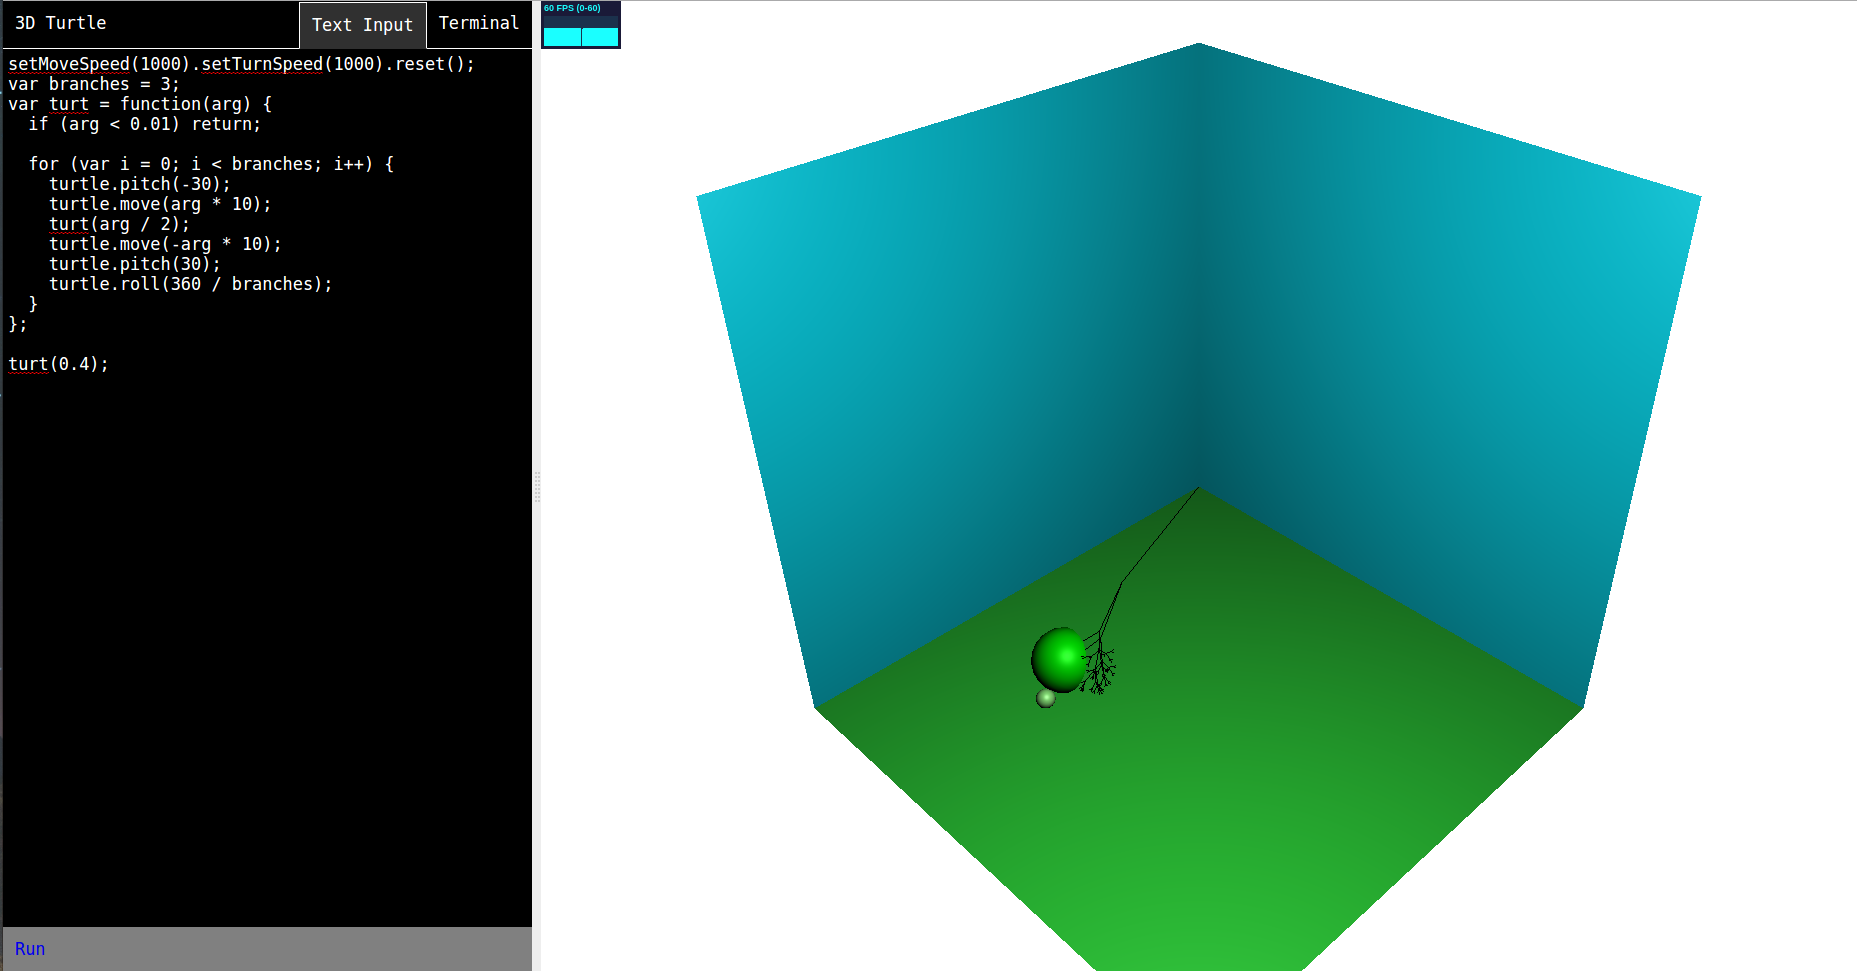
\includegraphics[width=\textwidth]{interface}
\caption{The user interface displaying a script in ``Text Input" mode and the turtle in the process of rendering from that script}
\end{figure}

\subsection{Application Overview}

The general procedure that this application will follow is

\begin{enumerate}
\item Receive input from the user and parse it into turtle commands
\item Execute those commands
\item Render the turtle
\end{enumerate}

For the first step, I opted to use JavaScript as the language with which the user will input commands. JavaScript offers a function \texttt{eval(...)} which takes a raw text string and interprets and executes it as JavaScript. By using JavaScript, a complete programming language, the user can take advantage of all of its constructs (loops, variables, conditionals, etc.) in a familiar way, and I, the developer, don't have to worry about reimplementing those things.

The user will have two ways to give the turtle commands, both of which emulate the options available in the familiar Python version of 2D turtle. The first is a basic implementation of a REPL (read-eval-print loop) terminal. Commands are entered and executed one line at a time. The second option allows general free-form text input; when the user clicks ``Run", the commands are executed as a whole unit. The first way is best for giving basic sequential commands; the second is ideal for writing complex scripts that feature things like loops and variables.

The turtle is represented as an instance of a class that is responsible for processing commands and rendering the resulting geometry. By default, there is a single turtle instance in the application. Each of that turtle's commands have a corresponding function in the global namespace that proxy the command through to that one turtle instance. That allows the user to type, for instance, \texttt{move(3)} instead of \texttt{turtle.move(3)}, which is more succinct and generally more convenient. This is best understood by reading the project's source code.

\subsection{Implementation of the Turtle}

The turtle is represented by a JavaScript class called Turtle. The class is designed to have minimal external dependencies, so it could easily be reused in other contexts. The turtle only depends on three.js for vector mathematics and rendering.

When a new instance of Turtle is instantiated, it creates a new scene into which it will put all the geometry it generates; that scene, in turn, is attached to a scene passed via the turtle's constructor.

Every command that the turtle receives immediately computes the turtle's new position and orientation and stores it; that new configuration is used to compute the turtle's new state for each subsequent command. That new computed orientation is not used immediately to render the turtle, however. To enable smooth animated moves, each new command is placed into a queue of commands. Those are processed one by one, and for each command, the turtle is smoothly interpolated between the starting and ending configurations of that command.

\subsection{Implementation of the User Interface}

There are three main components of the user interface: the portion that displays all turtles and a background, the "terminal" command interface, and the "text input" command interface. The interface is split horizontally into two panes: one for entering commands, and one for viewing the rendered output. Those two panes can be be resized by the user by dragging the divider between them.

The "terminal" command interface emulates a very basic terminal: commands are entered and processed one line at a time. Like you would expect, the user can use the up and down arrow keys to scroll through past commands. This terminal interface is a good way for beginners to enter commands, but is limited in its usefulness: it's difficult to do any complex scripting of the turtle's behavior, and correcting any mistakes requires starting again from the beginning.

The "text input" command interface is designed for more advanced users. It allows users to input complex multi-line programs. The input is parsed as JavaScript using the \texttt{eval(...)} function, so it's possible to use everything that JavaScript has to offer: variables, loops, functions, and more. Fixing mistakes is easy, as the user can just edit the appropriate line and run the program again.

\section{Applications}

A part of the project was exploring what was possible with a 3D turtle graphics system. Thanks to the fact that the turtle can be controlled with complex JavaScript programs, the turtle can be made to do some pretty interesting things, which are explored in more detail here.

\subsection{Wireframe Shapes}

A pretty clear application of this is generating the wireframe outlines of shapes. A cube is especially easy to draw, considering that it's composed of straight lines and right angles. I leave it as a creative exercise to the reader to write a simple program to draw a wireframe cube; alternatively, you can cheat and look at

\[\texttt{project/src/turtle\_scripts/wireframe\_cube.js}\]

in my project files.

\subsection{Recursive Fractals}

A common introductory exercise in standard 2D turtle is to use recursion to create fractal-like shapes. Logically, this process can be expanded into three dimensions. Some very nice tree-like structures can be created with recursion; if you were to add in some randomness to the program, the trees could probably be made to look very organic. For an example of a program that draws such trees, see

\[\texttt{project/src/turtle\_scripts/fractal.js}\]

\subsection{Parametric Lines}

Traditionally, the turtle has been a strictly relative cursor; that is, it can only be told to move or turn in relation to its current orientation. It had no concept of the absolute world in which it exists. However, if we allow ourselves to deviate from tradition, we can make the turtle do some very interesting things. Specifically, we can give it the ability to move to a particular, absolute position in its environment, which I did by adding the command \texttt{moveto(x,y,z)}.

If we now introduce a function to generate a sequence of $(x, y, z)$ coordinates, we can make the turtle trace out a parametric curve in space. For an implementation of such a program, as well as functions for some interesting curves, you can look at

\[\texttt{project/src/turtle\_scripts/parametric\_line.js}.\]

\subsection{Plotting Explicit Surfaces}

Another interesting thing we can do with a turtle is to plot any surface that is explicitly defined as a function of $x$ and $y$; that is, $z = f(x,y)$. To do this, we make two passes over the domain of the function. On the first pass, we increment x by the step size; for each step over x, we step through the entire range of y. On the second pass, we increment y by the step size; for each step over y, we step through the entire range of x. At each step, we move the turtle to the point $(x, y, f(x, y))$. Once we have completed both passes, the turtle will have traced out a good approximation of the surface. It is easiest to understand what is going on here by reading through code that implements this and then watching what the turtle does; an example implementation can be found in

\[\texttt{project/src/turtle\_scripts/surfaces.js}.\] 

\subsection{Plotting Parametric Surfaces}

We can reuse an idea from plotting explicit surfaces to plot parametric surfaces. That is, we will step over the range of the parameters $u, v$ and plot the coordinates $(x(u, v), y(u, v), z(u, v))$ as we go. Again, this process is best understood by reading through an example implementation, which can be found in

\[\texttt{project/src/turtle\_scripts/parametric\_surfaces.js}.\]

\section{Ideas for Future Extensions}

Naturally, with only a semester to complete this project, I didn't get a chance to do everything with it that I wanted. Perhaps some future Math 198 students will want to complete one or two of these for a mini-project:
\begin{itemize}
\item Expand API to approach feature parity with Python turtle
\item Implement undo functionality
\item Add syntax highlighting and code formatting to ``text input” mode
\item Mobile version?
\item Let camera fly along with the turtle
\item Use WebVR (http://webvr.info/) to provide support for Oculus Rift or Google Cardboard headsets
\item Finish \texttt{help()} function
\item Add more in-depth in-app documentation
\item When plotting surfaces with \texttt{moveto()}, compute normal and heading vectors so the turtle will sit tangent to the surface
\end{itemize}

\end{document}
